\section{Experiments}
\label{section:experiments}
We investigate the feasibility of online adversarial attacks by considering an online version of the challenging NoBox setting \citep{bose2020adversarial} in which the adversary must generate attacks without any access, including queries, to the target model $f_t$. Instead, the adversary only has access to a surrogate $f_s$ which is similar to $f_t$. In particular, we pick at random a $f_t$ and $f_s$ from an ensemble of pre-trained models from various canonical architectures. We perform experiments on the MNIST \cite{lecun-mnisthandwrittendigit-2010} and CIFAR-10 \cite{krizhevsky2009learning} datasets where we simulate a $\mathcal{D}$ by generating $1000$ permutations of the test set and feeding each instantiation to Alg.~\ref{alg:online_adv_attack}. In practice, online adversaries compute the value 
%$\mathcal{V}_i$ 
$\mathcal{V}_i=\ell(f_s(x'_i),y_i)$ 
of each data point in $\mathcal{D}$ by attacking $f_s$ using their fixed attack strategy
(where $\ell$ is the cross-entropy),
but the decision to submit the attack to $f_t$ is done using an online algorithm~$\mathcal{A}$ (see Alg.~\ref{alg:online_adv_attack}). 
As representative attack strategies, we use the well-known FGSM attack \citep{goodfellow2014explaining} and a universal whitebox attack in PGD \citep{madry2017towards}. 
We are most interested in evaluating the online fool rate, which is simply the ratio of successfully executed attacks against $f_t$ out of a possible of $k$ attacks selected by $\mathcal{A}$. Attacks are conducted with respect to the $\ell_\infty$- norm with $\gamma = 0.3$ for MNIST and $\gamma = 0.03125$ for CIFAR-10. The architectures used for $f_s$, $f_t$, and additional metrics (e.g. competitive ratios) can be found in \S\ref{appendix:additional_results}. 

% \setlength{\textfloatsep}{0pt}% Remove \textfloatsep
\cut{
\begin{minipage}[t]{.5\linewidth}
\vspace{0pt}  
    \begin{algorithm}[H]
    \small
    \textbf{Inputs:} Permuted Datastream:$\mathcal{D}_\pi$, \, Online Algorithm:$\mathcal{A}$, \, Surrogate classifier:$f_s$,\, Target classifier:$f_t$,\, Attack method:$\textsc{Att}$,\, Loss:$\ell$, \, Budget:$k$,\, 
    Fool rate: $F^{\mathcal{A}}_\pi=0$.
    \begin{algorithmic}[1]
    \FOR{$(x_i,y_i)$ in $\mathcal{D}_\pi$}
    \STATE $x_i' \leftarrow  \textsc{Att}(x_i)$ \hfill \COMMENT{// Compute the attack}
    \STATE $\mathcal{V}_i \leftarrow \ell(f_s(x_i'),y_i)$  \hfill \COMMENT{// Compute the estimate of $v_i$}
    \IF{$\mathcal{A}(\mathcal{V}_1,\ldots, \mathcal{V}_i,k) == \textsc{True}$}
    \STATE  $F^{\mathcal{A}}_\pi \leftarrow F^{\mathcal{A}}_\pi+\tfrac{\mathbf{1}\{f_t(x_i')\neq y_i\}}{k}$  \hfill\COMMENT{// Submit  $x_i'$ on $f_t$} 
    \ENDIF
    \ENDFOR
    \STATE \textbf{return:} $F^{\mathcal{A}}_\pi$ \hfill\COMMENT{// Note that $\mathcal{A}$ always submits $k$ attacks} 
    \end{algorithmic}
     \caption{\small Online Adversarial Attack}
     \label{alg:online_adv_attack}
    \end{algorithm}
\end{minipage}
}

\xhdr{Baselines} 
To evaluate the utility of picking adversarial examples using online algorithms we rely on two main baselines. First, we use a \textsc{naive} baseline--a lower bound on achievable performance--where the examples to attack are picked uniformly at random, and an upper bound with the \textsc{OPT} baseline where attacks, while crafted using $f_s$, are submitted by using the true value $v_i$ and thus utilizes $f_t$.% These baselines respectively give lower and upper bounds on the performance of an online algorithm. 
% In addition, we also use \textsc{Virtual}, \textsc{Optimistic}, and \textsc{Single-Ref} as baselines for single threshold online algorithms.
\setlength{\textfloatsep}{5pt}% Remove \textfloatsep
\begin{figure*}[t]
    \centering
    %\vspace{-2mm}
    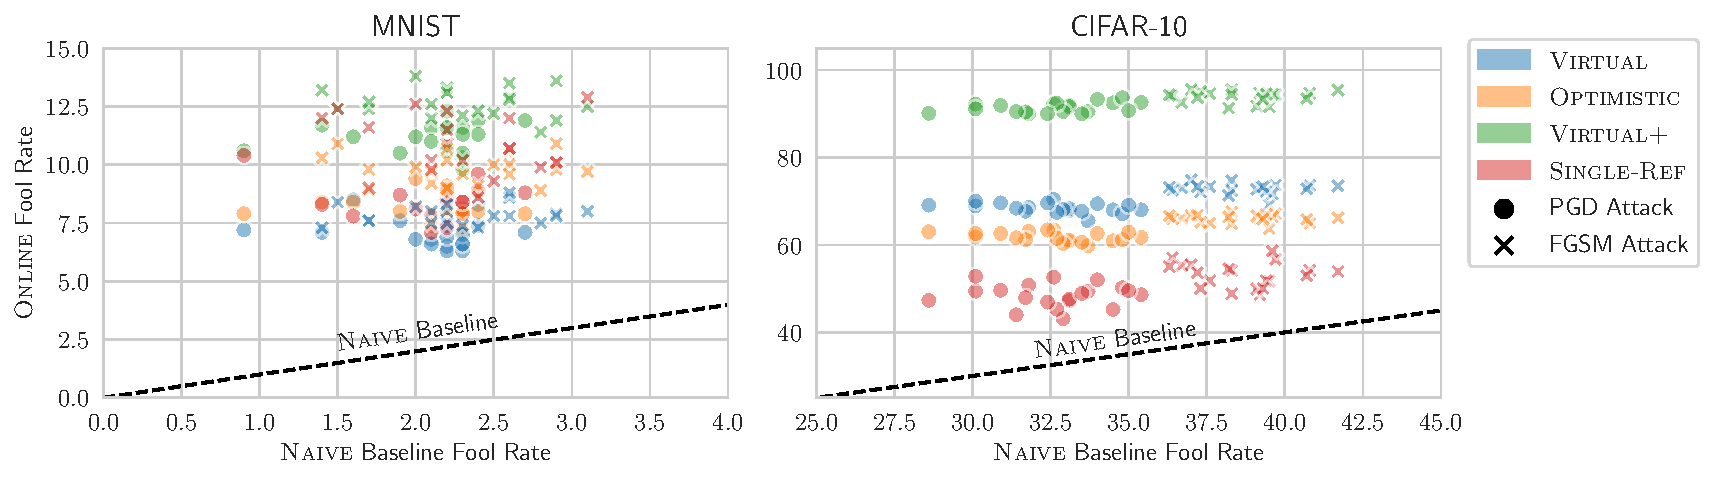
\includegraphics[width=.9\linewidth]{Figures/scatterplot_Q1.pdf}
    %\vspace{-4mm}
    \caption{ \small
    Plot of online fool rates for $k=1000$ against PGD-robust models using different online algorithms $\mathcal{A}$, attacks, datasets, and $20$ different permutations. For a given $x$-coordinate, a higher $y$-coordinate is better.} %The line $y=x$ corresponds to the \textsc{Naive} baseline.}
    \label{fig:scatter}
    %\vspace{-10pt}
\end{figure*}

\xhdr{Q1: Utility of using an online algorithm}
We first investigate the utility of using an online algorithm in selecting data points to attack in comparison to the \textsc{Naive} baseline. For a given permutation $\pi$ and an attack method (FGSM or PGD), we compute the online fool rate of the \textsc{Naive} baseline and online algorithms as $F^{\textsc{Naive}}_\pi$, $F^{\mathcal{A}}_\pi$ respectively. In Fig.~\ref{fig:scatter}, we uniformly sample $20$ permutations $\pi_i \sim \mathcal{S}_n, \, i \in [n],$ of $\mathcal{D}$ and plot a scatter graph of points with coordinates $(F^{\textsc{Naive}}_{\pi_i}, F^{\mathcal{A}}_{\pi_i})$, for different online algorithms $\mathcal{A}$, attacks with $k=1000$,\footnote{\small \url{https://github.com/MadryLab/[x]_challenge}, for $\texttt{[x]} \in \texttt{\{MNIST, CIFAR10 \}}$ .} and datasets. The line $y=x$ corresponds to the \textsc{Naive} baseline performance ---i.e. points with coordinates $(F^{\textsc{Naive}}_\pi, F^{\textsc{Naive}}_\pi)$---and each point above that line corresponds to an online algorithm that outperforms the naive baseline on a specific permutation $\pi_i$. As observed, all online algorithms significantly outperform the \textsc{Naive} baseline, on sampled $\pi_i$'s with an average aggregate improvement of 7.5\% and 34.1\% on MNIST and CIFAR-10.


\begin{table*}[ht]
%\vspace{-10pt}
%\begin{small}
\small
\caption{Online fool rate on non-robust models using FGSM and PGD attacker and various online algorithms. For a given attack and value of $k$: {\color{g1} $\mathbf{\bullet}$ } at least 97\%,
\textbf{\color{g2} $\mathbf{\bullet}$} at least 95\%, \textbf{\color{g3}$\mathbf{\bullet}$} at least 90\%, \textbf{\color{g4} $\mathbf{\bullet}$} less than 90\% of the optimal performance achievable given by \textsc{Opt} in \textbf{bold}.}
\label{table:non_robust_table1}
 \begin{center}\begin{tabular}{ c c c c c c c c }
 \toprule
 & & \multicolumn{3}{c}{MNIST (Online fool rate in \%)} & \multicolumn{3}{c}{CIFAR-10 (Online fool rate in \%)}\\
%  \cmidrule{3-8}
 & Algorithm & $k=10$ & $k=100$ & $k=1000$ & $k=10$ & $k=100$ & $k=1000$ \\
 \midrule
 \multirow{6}{*}{\rotatebox[origin=c]{90}{FGSM}}
 %\multirow{6}{*}{FGSM}
 & \textsc{Naive}& 64.1 $\pm$ 32.2 & 47.8 $\pm$ 30.7 & 45.7 $\pm$ 30.7 & 60.7 $\pm$ 16.1 & 59.2 $\pm$ 6.2 & 59.2 $\pm$ 4.3\\
 & \textsc{Opt}  & \textbf{87.0 $\pm$ 0.5} & \textbf{84.7 $\pm$ 0.5} &  \textbf{83.6 $\pm$ 0.4} & \textbf{86.6 $\pm$ 0.4} & \textbf{87.3 $\pm$ 0.3} &  \textbf{86.5 $\pm$ 0.2} \\
 \cmidrule{2-8}
 %\bottomrule
 %& \textsc{Best Online} & \cellcolor{g1} 76.3 $\pm$ 27.6 & 55.0 $\pm$ 28.8 & 52.9 $\pm$ 26.7\\
 %& \textsc{Worst Online} & \cellcolor{g3} 69.8 $\pm$ 31.9 & 52.6 $\pm$ 29.7 & 49.0 $\pm$ 28.7 \\
 %  \cmidrule{2-8}
 & \textsc{Optimistic} & \cellcolor{g3}79.0 $\pm$ 0.5 & \cellcolor{g3}77.6 $\pm$ 0.4 &\cellcolor{g3} 75.3 $\pm$ 0.4 &\cellcolor{g4} 75.3 $\pm$ 0.5 & \cellcolor{g4} 72.8 $\pm$ 0.2 &\cellcolor{g4} 71.9 $\pm$ 0.2\\
 & \textsc{Virtual} & \cellcolor{g3}78.6 $\pm$ 0.5 &\cellcolor{g3} 79.1 $\pm$ 0.4 &\cellcolor{g3} 77.4 $\pm$ 0.4 & \cellcolor{g4} 76.1 $\pm$ 0.5 &\cellcolor{g4} 77.1 $\pm$ 0.2 & \cellcolor{g4}75.4 $\pm$ 0.2\\
 & \textsc{Single-Ref} &\cellcolor{g2}85.1 $\pm$ 0.5 & \cellcolor{g1}83.0 $\pm$ 0.5 &\cellcolor{g4} 72.3 $\pm$ 0.5 &\cellcolor{g3} 80.4 $\pm$ 0.5 &\cellcolor{g2} 84.0 $\pm$ 0.3 & \cellcolor{g4}66.0 $\pm$ 0.2\\
 & \algoname & \cellcolor{g3}80.4 $\pm$ 0.5 &\cellcolor{g1} 82.5 $\pm$ 0.4 & \cellcolor{g1} 82.9 $\pm$ 0.4 &\cellcolor{g2} 82.9 $\pm$ 0.5 & \cellcolor{g1}86.3 $\pm$ 0.3 &  \cellcolor{g1}85.2 $\pm$ 0.2\\
 \midrule
 %\multirow{6}{*}{PGD}
  \multirow{6}{*}{\rotatebox[origin=c]{90}{PGD}}
 & \textsc{Naive} & 69.7  $\pm$ 15.6 & 67.2 $\pm$ 19.1 & 67.9 $\pm$ 17.4 & 72.5 $\pm$ 17.6 & 70.4 $\pm$ 9.4 & 68.6 $\pm$ 6.3\\
 & \textsc{Opt} & \textbf{73.6 $\pm$ 0.9} & \textbf{49.8 $\pm$ 0.8} & \textbf{49.6 $\pm$ 0.8} & \textbf{83.7 $\pm$ 0.6} & \textbf{80.6 $\pm$ 0.6} & \textbf{79.9 $\pm$ 0.5}\\
 \cmidrule{2-8}
 %\bottomrule
 & \textsc{Optimistic} & \cellcolor{g3} 66.2 $\pm$ 1.1 & \cellcolor{g2} 48.2 $\pm$ 0.8 &\cellcolor{g3} 45.1 $\pm$ 0.9 &\cellcolor{g3} 79.1 $\pm$ 0.6 & \cellcolor{g3}76.6 $\pm$ 0.4 & \cellcolor{g3}76.0 $\pm$ 0.4\\
 & \textsc{Virtual} &\cellcolor{g4} 63.4 $\pm$ 1.1 & \cellcolor{g4}46.2 $\pm$ 0.9 &\cellcolor{g2} 46.8 $\pm$ 0.8 & \cellcolor{g3}78.3 $\pm$ 0.6 &\cellcolor{g3} 77.5 $\pm$ 0.5 &\cellcolor{g3} 76.9 $\pm$ 0.4\\
 &\textsc{Single-Ref} & \cellcolor{g1} 71.5 $\pm$ 0.9 & \cellcolor{g1} 49.7 $\pm$ 0.8 & \cellcolor{g4}42.9 $\pm$ 0.9 & \cellcolor{g2}80.2 $\pm$ 0.6 &\cellcolor{g1} 79.6 $\pm$ 0.5 & \cellcolor{g4} 74.5 $\pm$ 0.4\\
 & \algoname         &\cellcolor{g2} 68.2 $\pm$ 1.0 & \cellcolor{g1}49.3 $\pm$ 0.8 & \cellcolor{g1} 49.7 $\pm$ 0.8 & \cellcolor{g1} 81.2 $\pm$ 0.6 & \cellcolor{g1} 80.1 $\pm$ 0.6 &\cellcolor{g1}79.5 $\pm$ 0.5\\
 \bottomrule
\end{tabular}\end{center} 
%\end{small}
%\vspace{-15pt}
\end{table*}


\xhdr{Q2: Online Attacks on Non-Robust Classifiers}
While previous work on online algorithms focused largely on the theoretical contribution, we are equally interested in their performance in practical applications, where the assumptions of the theory may not necessarily hold anymore. We thus decide to propose the first comparison of online algorithms in the context of attacking non-robust MNIST and CIFAR-10 classifiers.  We report the average performance of all online algorithms, \algoname\ with $t=\alpha^* n$ as in Eq.~\ref{eq:alpha_eqn}, and the optimal offline algorithm \textsc{Opt} in Tab.~\ref{table:non_robust_table1}. For MNIST, we find that the two best online algorithms are \textsc{Single-Ref} and our proposed \algoname\ which approach the upper bound provided by \textsc{Opt}. For $k=10$ and $k=100$, \textsc{Single-Ref} is slightly superior while $k=1000$ \algoname\ is the best method with an average relative improvement of $15.3\%$. This is unsurprising as \algoname\ does not have any additional hyperparameters unlike \textsc{Single-Ref} which appears more sensitive to the choice of optimal thresholds and reference ranks, both of which are unknown beyond $k=100$ and non-trivial to find in closed form (see \S\ref{appendix:additional_results_larger_datasets} for details). On CIFAR-10, we observe that \algoname\ is the best approach regardless of attack strategy and the online attack budget $k$. A notable observation is that even relatively simple and common attack strategies like FGSM and PGD can be turned into very strong transfer attack strategies when paired with an appropriate $\mathcal{A}$, highlighting the importance of carefully choosing data points to attack in the online setting. %as a significant factor in achieving high online fool rates. 


\begin{table*}[ht]
\small
\caption{Online fool rate on robust models using FGSM and PGD attacker and various online algorithms. For a given attack and value of $k$: {\color{g1} $\mathbf{\bullet}$ } at least 90\%,
\textbf{\color{g2} $\mathbf{\bullet}$} at least 80\%, \textbf{\color{g3}$\mathbf{\bullet}$} at least 70\%, \textbf{\color{g4} $\mathbf{\bullet}$} less than 70\% of the optimal performance achievable given by \textsc{Opt} in \textbf{bold}.}
\label{table:madry_challenge}
 \begin{center}\begin{tabular}{ c c c c c c c c}
 \toprule
 & & \multicolumn{3}{c}{MNIST (Online fool rate in \%)} & \multicolumn{3}{c}{CIFAR-10 (Online fool rate in \%)}\\
%   \cmidrule{3-8}
 & Algorithm & $k=10$ & $k=100$ & $k=1000$ & $k=10$ & $k=100$ & $k=1000$ \\
 \midrule 
 %\multirow{6}{*}{FGSM}
 \multirow{6}{*}{\rotatebox[origin=c]{90}{FGSM}}
 & \textsc{Naive} & $2.1 \pm 4.5$ & $2.1 \pm 1.4$ & $2.1 \pm 0.4$ & 31.9 $\pm$ 14.2 & 32.6 $\pm$ 4.7 & 32.5 $\pm$ 1.5\\
 & \textsc{Opt} & \textbf{80.0 $\pm$ 0.0} & \textbf{55.0 $\pm$ 0.0} & \textbf{18.9 $\pm$ 0.0} & \textbf{100.0 $\pm$ 0.0} & \textbf{100.0 $\pm$ 0.0} & \textbf{97.2 $\pm$ 0.0}\\
 \cmidrule{2-8}
 & \textsc{Optimistic} & \cellcolor{g3}$49.7 \pm 0.6$ & \cellcolor{g4}$25.7$ $\pm$ $0.1$ &\cellcolor{g3} $9.7$ $\pm$ $0.0$ & \cellcolor{g2}72.4 $\pm$ 0.5 & \cellcolor{g3}64.6 $\pm$ 0.1 & \cellcolor{g3}61.9 $\pm$ 0.0\\
 & \textsc{Virtual} & \cellcolor{g3}49.8 $\pm$ 0.5 & \cellcolor{g3}27.8 $\pm$ 0.1 &\cellcolor{g4} 8.1 $\pm$ 0.0 & \cellcolor{g2}75.1 $\pm$ 0.5 & \cellcolor{g3}74.3 $\pm$ 0.1 & \cellcolor{g2}68.9 $\pm$ 0.0\\
 & \textsc{Single-Ref} & \cellcolor{g2}62.0 $\pm$ 0.7 & \cellcolor{g2}45.2 $\pm$ 0.2 & \cellcolor{g3}10.2 $\pm$ 0.0 & \cellcolor{g2}84.3 $\pm$ 0.6 & \cellcolor{g1}90.9 $\pm$ 0.3 &\cellcolor{g4} 48.6 $\pm$ 0.1\\
 & \algoname & \cellcolor{g2}68.2 $\pm$ 0.5 & \cellcolor{g2}42.2 $\pm$ 0.1 & \cellcolor{g3}{12.7 $\pm$ 0.0} & \cellcolor{g1}91.5 $\pm$ 0.4 & \cellcolor{g1}96.5 $\pm$ 0.1 & \cellcolor{g1}{91.7 $\pm$ 0.0}\\
 \midrule
 %\multirow{6}{*}{PGD}
 \multirow{6}{*}{\rotatebox[origin=c]{90}{PGD}}
 & \textsc{Naive} & 1.8 $\pm$ 4.1 & 1.9 $\pm$ 1.4 & 1.9 $\pm$ 0.4 & 39.1 $\pm$ 14.2 & 38.9 $\pm$ 4.4 & 38.7 $\pm$ 1.5\\
 & \textsc{Opt} & \textbf{58.9 $\pm$ 0.4} & \textbf{39.9 $\pm$ 0.1} & \textbf{16.1 $\pm$ 0.0 }& \textbf{100.0 $\pm$ 0.0} & \textbf{100.0 $\pm$ 0.0} & \textbf{98.0 $\pm$ 0.0}\\
 \cmidrule{2-8}
 & \textsc{Optimistic} & \cellcolor{g2}34.9 $\pm$ 0.5 & \cellcolor{g4}19.2 $\pm$ 0.1 &\cellcolor{g3} 8.2 $\pm$ 0.0 & \cellcolor{g2}75.4 $\pm$ 1.9 & \cellcolor{g3}68.5 $\pm$ 0.4 & \cellcolor{g3}66.0 $\pm$ 0.1\\
 & \textsc{Virtual} & \cellcolor{g2}35.4 $\pm$ 0.5 & \cellcolor{g3}21.8 $\pm$ 0.1 &\cellcolor{g4} 7.2 $\pm$ 0.0 & \cellcolor{g2}78.1 $\pm$ 1.7 &\cellcolor{g2} 77.3 $\pm$ 0.5 & \cellcolor{g2}72.8 $\pm$ 0.1\\
 & \textsc{Single-Ref} &\cellcolor{g1} 44.1 $\pm$ 0.6 & \cellcolor{g2}33.9 $\pm$ 0.2 & \cellcolor{g3}8.3 $\pm$ 0.0 & \cellcolor{g2}86.2 $\pm$ 2.2 &\cellcolor{g1} 91.9 $\pm$ 0.9 & \cellcolor{g3}53.2 $\pm$ 0.3\\
 & \algoname & \cellcolor{g1}48.3 $\pm$ 0.5 & \cellcolor{g2}32.8 $\pm$ 0.1 & \cellcolor{g3}11.1 $\pm$ 0.0 & \cellcolor{g1}92.2 $\pm$ 1.3 & \cellcolor{g1}97.1 $\pm$ 0.4 &\cellcolor{g1} 94.2 $\pm$ 0.1\\
 \bottomrule
\end{tabular}\end{center} 
%\vspace{-15pt}
\end{table*}


\xhdr{Q3: Online Attacks on Robust Classifiers}
We now test the feasibility of online attacks against classifiers robustified using adversarial training. To do so, we adapt the public Madry Challenge \citep{madry2017towards} to the online setting, by attacking a subset of the test set as it is streamed. We report the average performance of each online algorithm in Table ~\ref{table:madry_challenge}. We observe that \algoname\ (with $t$ as in Eq.~\ref{eq:alpha_eqn}) is the best online algorithms, outperforming \textsc{Virtual} and \textsc{Optimistic}, in all settings except for $k=10$ on MNIST where \textsc{Single-Ref} is slightly better. An interesting observation for CIFAR-10 is that attacks on robust models in comparison to non-robust models lead to higher success rates in the online setting. We reconcile this counter-intuitive fact by noting that even when $k=1000$, it corresponds to only $10\%$ of the test set while a PGD-attack can transfer with 38.7\%  efficacy on the robust model for the entire test set. Thus, the efficiency of an online attacks requires the ability to detect the optimal examples to attack than the global robustness of a model which is highly influenced by the distribution of $\mathcal{V}_i$. For instance, if the value of the examples that correspond to a successful attack cannot be distinguished from the ones that are unsuccessful, then one cannot hope to use an online algorithm---that only observe values---to always manage to pick successful attacks.
% for non-robust models, there may be many equally attackable, but potentially low-value datapoints ---i.e. the distribution of $\mathcal{V}_i$'s is flat. 
% Thus attacking these points might not result in transferable attack vectors against $f_t$. 
% On the other hand, for robust models, there are fewer attackable points and attacking via selections of an online algorithm lead to higher transfer rates on $f_t$. 
We empirically verify that these distributions of values $\mathcal{V}_i$ for CIFAR-10 robust and non-robust models are relatively different in \S\ref{appendix:visualization_of_values_observed}.






